\chapter{Key Concepts}
\section{URC}
Ultra reliable communication (URC) is a concept, that will be introduced with the new 5G Wireless Systems. (Petar) It is one's of the new features that will come with the 5G network. The 4G network and 4G LTE network works with a block/bit error rate on $10^{-3}$, which is a very normal standard of error rate. But URC introduces a error rate on $10^{-5}$-$10^{-6}$. This of course comes with cost of either higher signal needed to be send, to get a higher signal-to-noise ratio (SNR) or lower bit rates, to introduce more error coding. But the return of this, a higher reliability and a lower latency is introduced. By having this two features introduced, more automatic and/or high precision machines can be connected to the network. An example is the use of the cellular network, to get self-driving cars to communicated with each other. In the case, that a car have to make a fast braking action, this have to be communicated to the cars behind it, with high reliability and low latency. So be introducing this URC, the cellular network can be used for more than just communication between humans, but also for fast and precises communication between machines.

\section{Diversity}
Diversity is used to combat fading in a wireless system. By using clever techniques you can effectively deliver several copies or replicas of a signal to the receiver. There is a lower chance that all of these copies of signals are going to have a deep fade at the same time \citep[p. 4-6]{diversityFuture}. The overall goal is to provide a gain in signal quality by having several signals that independently fade from each other without the cost of more power consumption, reduced bit rate and complexity or other resources. There are several ways to achieve diversity in a wireless system. \\
Time diversity: By retransmitting the same information you get some diversity gain on the cost of decreased bit/rate. Usually a forward error correction code is added instead of just re transmitting the signals several times. \\
Antenna diversity / Spatial diversity
By having several antennas at both/or the receiver and transmitter a antenna diversity is achieved. With several antennas the signal can be combined together to process the signals into one. To get independently fading signals the signals need to be uncorrelated by separating the antennas least half a wavelength (micro diversity) \citep{diversityAntenna}. Antenna diversity comes at the cost of having to power more than one antenna.


\section{Dynamic range}
Dynamic range in RF systems is the ability of the receiver to pick out weak signals compared to the strong ones(the range of the low signals to the high signals which the receiver can operate). Think about it as trying to hear a person talking when somebody in the room is screaming. For Network analysers the dynamic range is the maximum signal power the receiver can measure minus the noise floor of the receiver. To achieve a higher dynamic range of NVAs it must be  in tuned-receiver mode (Narrowband). If you reduce the bandwidth then the overall noise floor will go down, so it logical that it would have higher dynamic range. \citep{AgilentNVA} \\
In a normal receiver the dynamic range goes from the Third order intercept point and the sensitivity of the receiver(the dynamic range is set by the sensitivity of the receiver to the Third order intercept point). Third order intercept points are caused by over driving the receiver with too much input and that causes distortion and signal saturation. The sensitivity is more dependent on the operating environment and the receivers noise figure. \citep{understandDynamic} This means that a RF receiver is highly dependent on the mixer and amplifier with regards to dynamic range.\\
To measure with high dynamic ranges a special measurement setup would be required to increase the dynamic range.
Measuring a very narrow bandwidth

Averaging the noise so that the variance is reduced (but longer measuring time).

\begin{figure}[H]
\centering
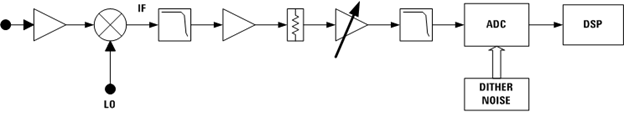
\includegraphics[width=0.65\textwidth]{figures/Block_VNA.png}
\caption{A Typical block diagram of a VNA receiver.}
\label{fading_gain}
\end{figure}

Given the noise is uncorrelated, by averaging the measured(complex) data the noise component will approach zero.That means that our end signal in the output will be with less noise.Every time that our average is getting double, the signal to noise ratio is increased by 3dB .The problem is that by averaging the double of every measured data will take twice as long.\citep{KeysightAVG}


The setup of the VNA measuring would have to take into account some factors to increase the dynamic range and have it be accurate. \\
The intermediate frequency is a frequency that shifted to in order to easier process the signal. This is done in the first stages of a receiver. This frequency is normally lower than the transmitted RF frequency, this epically helps the ADC that uses a lower sampling rate. 
By setting the IF filter to a very narrow bandwidth (narrowband) the noise floor goes down and increases the dynamic range. The cost of using a narrowband is the measurement time, as the NVA would need several sweeps to cover a typical bandwidth.

Dynamic Accuracy/range is effected by the non-linearity in the receiver chain, the worst part being the mixers and amplifiers since they introduce the most non-linearity. To measure the linearity of a receiver a power change measurements is preformed and compared to a reference level of power change that is accurate. This means that the linearity of a receiver as can be defined as LA =receiver measured power change / reference power change.
Cross talk is the energy leakage between signal paths of the measuring system and this becomes a problem in high-loss transmission measurements. This is can be fixed by running an Isolation calibration \citep{crosstalk}. This accrues below the noise floor so averaging and low IF bandwidth must be used during calibration.
At low power levels <-70dBm the main non-linearity comes from the analog to Digital converter. Quantizing error causes this when converting analog signals. The ADC used in NVA are top of the line and can use a Gaussian noise ditcher to combat the non linear nature of a ADC. 



\section{Rayleigh Fading}
\section{Statistics}
\subsection{Confidence Interval}
\subsection{Distributions?}